\section{Grid Computing}
Grid computing \cite{li2005grid} is the most recent decade's technology innovation in high performance computing. A large number of scientists working on the operations of this huge co-operative project of EU. Monitoring \& information architecture \cite{fisher2002datagrid} has been standardized in the initial state of that project, to succeed in today scale of 150.000 cores in production. Use of grid computing nowadays takes place in academic and research environments. Also, applications in industry-based needs such as promising Power Grid control \cite{Taylor2006} are emerging.

Grid computing may be the infrastructure over which Cloud Computing may reside. Cloud computing promise that it will change how services are developed, deployed and managed. The elastic demands of education and research community is a good place where cloud computing may be developed. Many datacenters all over Europe which are currently serving grid computing infrastructure for LHC, could later share the resources to help some other big academic projects scale up as needed.

\section{Resource Brokers}
Resource Brokers \cite{Kertesz06ataxonomy} where developed to manage the workload on Computer elements and Resource elements. Globus is a non-service based RB, and gLite RB which is service based. A Workload Management System (WMS) exists in gLite to do the distribution and management of the Computing and Storage oriented tasks.

Based on the middleware that resource brokers rely on, they use the equivalent information system. From resource broker's point of view, the relevant information is the data store and query. There are two main categories of information systems in middlewares. The Directory-based and the Service-based. They are used for resource mapping by the brokers when they access the resource data.

\begin{figure}[h]
\begin{center}
% Set the overall layout of the tree
\tikzstyle{level 1}=[level distance=3.5cm, sibling distance=3.5cm]
\tikzstyle{level 2}=[level distance=3.5cm, sibling distance=2cm]

% Define styles for bags and leafs
\tikzstyle{bag} = [text width=4em, text centered, circle, thick]
\tikzstyle{end} = [circle, minimum width=3pt,fill, inner sep=0pt]

% The sloped option gives rotated edge labels. Personally
% I find sloped labels a bit difficult to read. Remove the sloped options
% to get horizontal labels. 
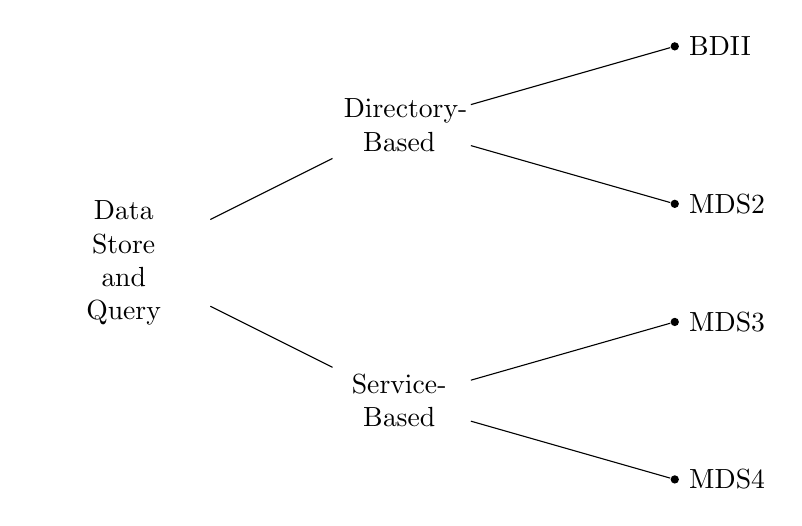
\begin{tikzpicture}[grow=right, sloped]
\node[bag] {Data Store and Query}
    child {
        node[bag] {Service-Based}        
            child {
                node[end, label=right:
                    {MDS4}] {}
                edge from parent
                node[above] {}
                node[below]  {}
            }
            child {
                node[end, label=right:
                    {MDS3}] {}
                edge from parent
                node[above] {}
                node[below]  {}
            }
            edge from parent 
            node[above] {}
            node[below]  {}
    }
    child {
        node[bag] {Directory-Based}        
        child {
                node[end, label=right:
                    {MDS2}] {}
                edge from parent
                node[above] {}
                node[below]  {}
            }
            child {
                node[end, label=right:
                    {BDII}] {}
                edge from parent
                node[above] {}
                node[below]  {}
            }
        edge from parent         
            node[above] {}
            node[below]  {}
    };
\end{tikzpicture}
\caption{Grid Resource Brokers grouped by Information Systems\cite{Kertesz06ataxonomy}}
\end{center}
\end{figure}

\subsection{Globus}

Globus Toolkit is an open source toolkit used to build grids. It provides standards such as OGSA, OGSI, WSRF and GSI, and the implementations of OGF protocols such as MDS and GRAM.

\nomenclature{OGF}{Open Grid Forum}
\nomenclature{OGSA}{Open Grid Services Architecture}
\nomenclature{OGSI}{Open Grid Services Infrastructure}
\nomenclature{WSRF}{Web Services Resource Framework}
\nomenclature{MDS}{Monitoring and Discovery Service}
\nomenclature{GRAM}{Grid Resource Allocation \& Management Protocol}
\nomenclature{GSI}{Grid Security Infrastructure}

\begin{figure}[htb]
\centering
 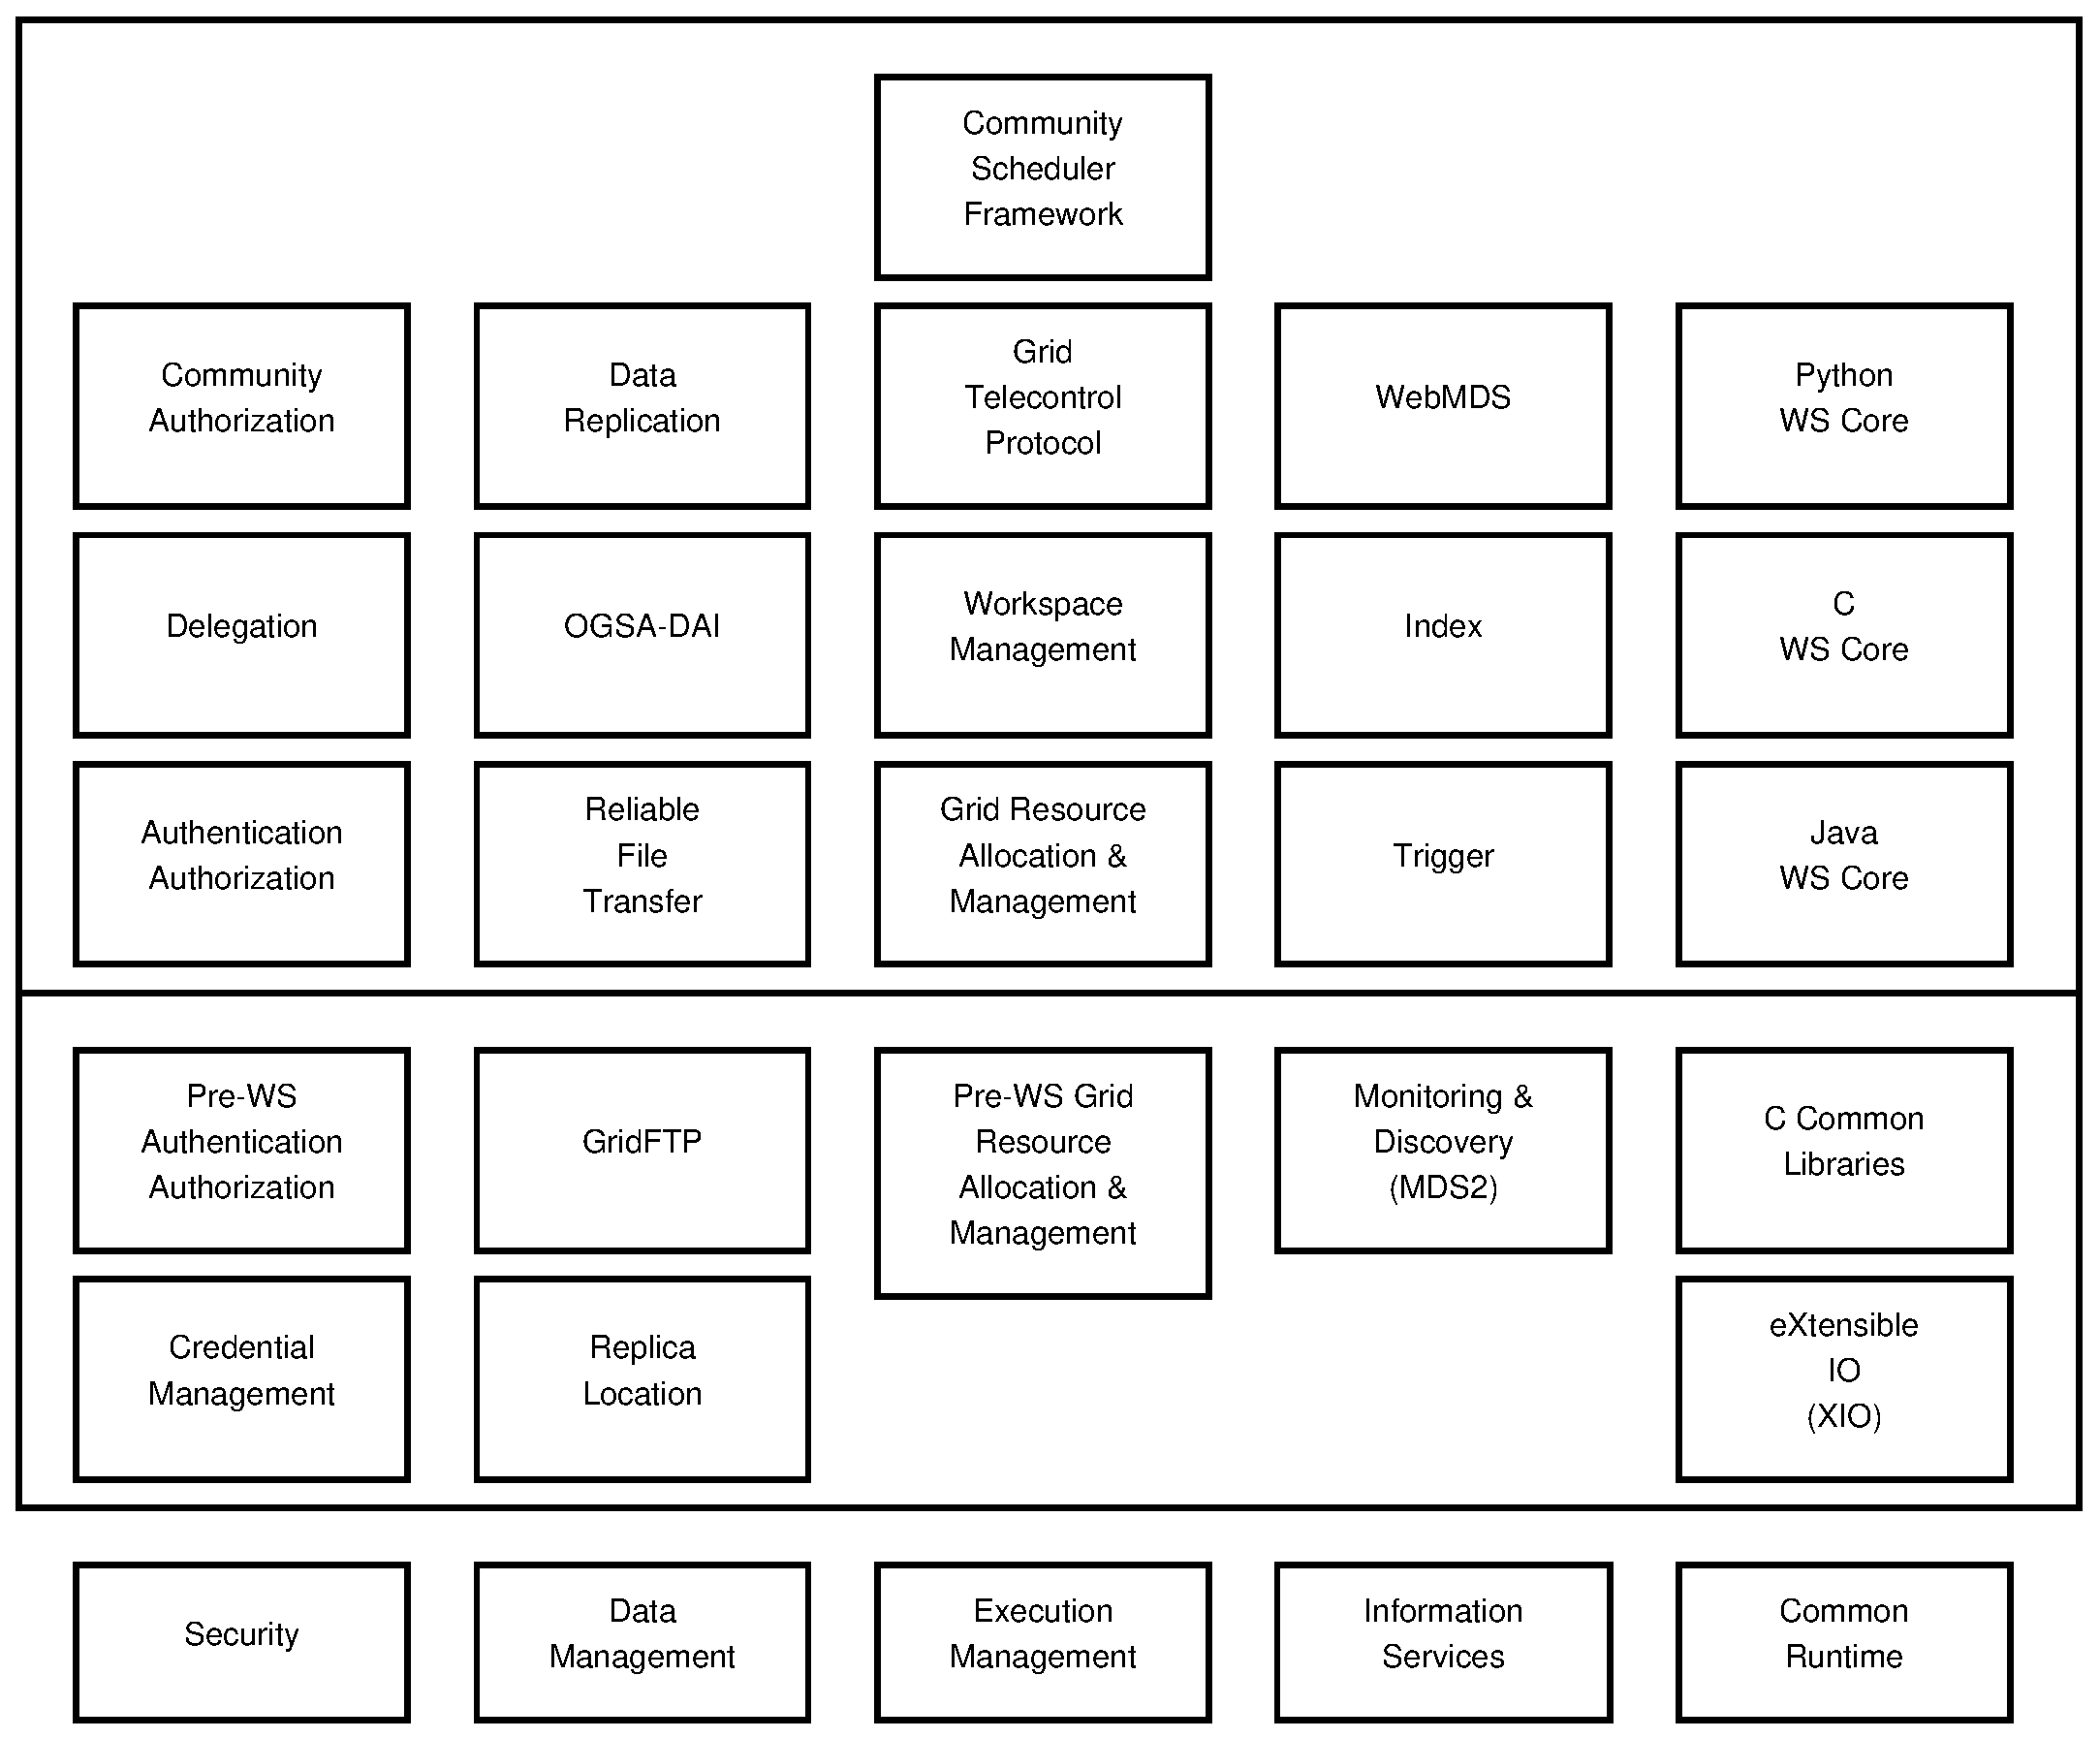
\includegraphics[width=6in]{images/globus.eps}
\caption{Globus Toolkit version 4 (GT4)}
\label{figure:globus}
\end{figure}

Monitoring and Discovery Service (MDS) is part of Globus Toolkit, and provides the information for the availability and status of grid resources. As a suite of Web Services, it offers a set of components that help to the discovery and monitoring of the resources that are available to a Virtual Organization.

\subsection{gLite}

gLite is a middleware which was created to be used in the operation of the experiment LHC in CERN. The user community is grouped in Virtual Organizations, and the security model is GSI. A grid using gLite consists of User Interface, Computer Element, Storage Element, Workload Management System and Information Service.

The information service in version 3.1 of gLite is similar to MDS of Globus middleware, except that the GRIS and GIIS are provided by BDII (see Section \nameref{subsec:BDII}) which is an LDAP based service.

\nomenclature{BDII}{Berkeley Database Information Index}


%% TODO more about glite

\section{Information Services}
\begin{figure}[htb]
\centering
 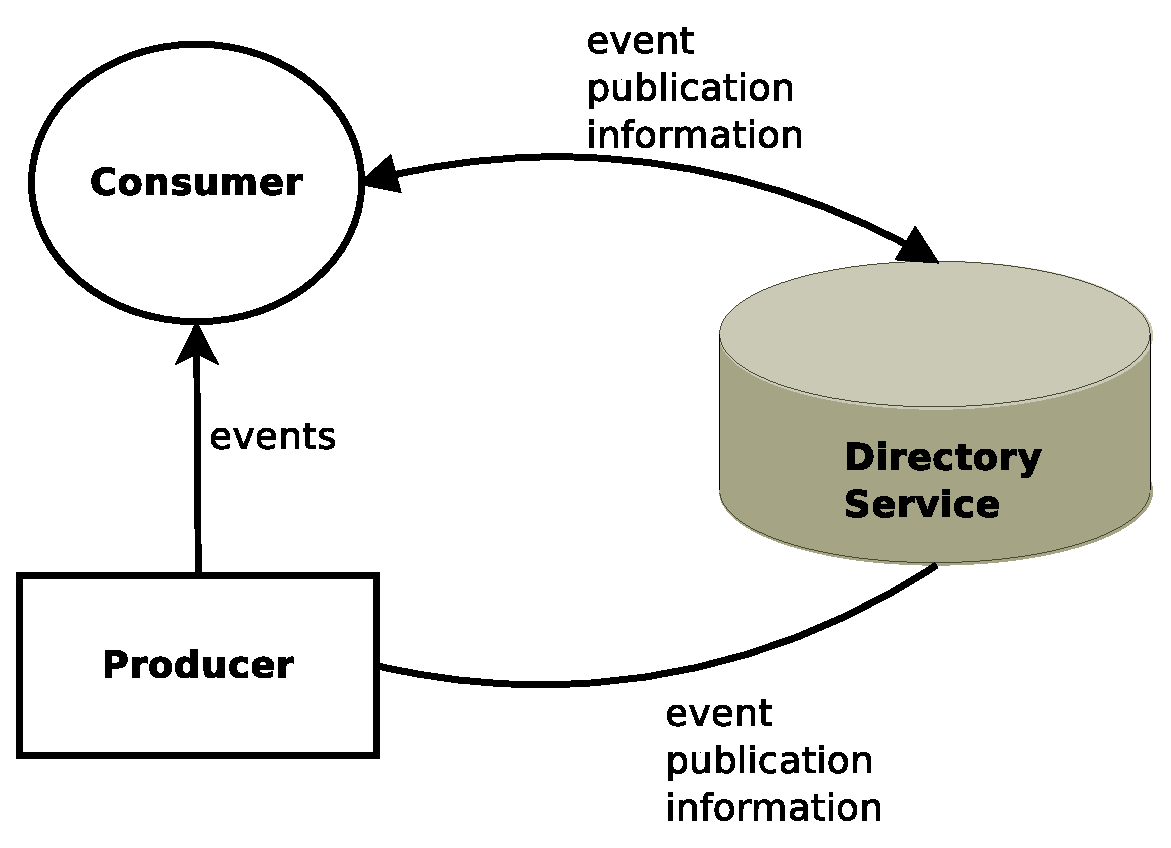
\includegraphics[width=4in]{images/gma.eps}
\caption{Grid Monitoring Architecture}
\label{figure:gma}
\end{figure}
A Grid Monitoring Architecture \cite{tierney2002grid} was proposed in early 2000's. Information systems were developed to create repositories of information needed to be stored for monitoring and statistical reporting reasons. Such an organized system later was specified by the Aggregated Topology Provider (ATP) definition. The largest world grids adopt that model, forming OIM in OSG (USA) and GOCDB as that information base in EGEE (Europe). Message Bus was also defined as a mean to transfer the underlying data, and well known tools came up such as Gstat, GOCDB and BDII with Glue specification. Grid performance monitoring and keeping of such an information system has also impact in the performance of the system it shelf \cite{zhang2003performance}, so various methods were developed to give the solution to the scaling and performance problem, such as MDS2 (GIIS \& GRIS), GMA and R-GMA \cite{wilson2004information}, which offers relational environment \cite{fisher2001relational}, has experience on production systems \cite{byrom-production} and scales to reach huge needs such as CMS project \cite{Bonacorsi2004,Byrom}.

\subsection{MDS}
Monitoring and Discovery Services is about collecting, distributing, indexing and archiving information of the status of resources, services and configurations. The collected information is used to detect new services and resources, or to monitor the state of a system.

Globus Toolkit was using LDAP-based implementation for its information system since its early versions, back in 1998 \cite{von1998usage}. MDS2 in Globus Toolkit fully implemented referral with a combined GRIS and GIIS, using mds-vo-name=local to refer to the GRIS and all other strings to refer to a GIIS. It was widely accepted as a standard implementation of a grid information system \cite{945188}, with good scalability and performance \cite{zhang2004performance}.

\nomenclature{GIIS}{Grid Index Information Service}
\nomenclature{GRIS}{Grid Resource Information Service}

MDS 4 consists of the Web Services Resource Framework and a web service data browser, WebMDS. The WSRF Aggregator Framework includes:

\begin{enumerate}
  \item MDS-Index, which provides a collection of services monitoring information and an interface to query such information.
  \item MDS-Trigger, which provides a mechanism to take action on collected information.
  \item MDS-Archive, is planned for future release of MDS, to provide access to archived data of monitoring information.
\end{enumerate}

External software components that are used to collect information (such as Ganglia)\cite{gangliaWSRF} are called Information Providers.


\subsection{Glue}
As long as Information Services are used to connect different infrastructures, the schema of its structure had to be standardized. To inter-operate EU and USA grids, DataTAG developed the GLUE schema implementation. GLUE specification quickly adopted by the communities and currently its recommended LDAP DIT is specified in GLUE specification v.$2.0$ from GLUE Working Group of OSG.

Many objectclasses of the Glue schema define a Computer Element, a Storage Element, etc. As seen in Figure \ref{figure:gluece_ext} in later chapter, performance monitoring attributes such as processor load are defined in objectclasses that extends Computer Element objectclass.

\subsection{BDII}\label{subsec:BDII}
BDII is used by gLite as the Information Index Service of the LHC experiment. It is LDAP based and may be at top-level or site-level. The GIIS has been replaced by site BDII, which is fundamental for a site in order to be visible in the grid.

Top-level BDII contains aggregated information about the sites and the services they provide. Site BDII collects the information from its Computer Elements, Storage Elements, etc as long as every configured service that is installed on the site.

Information about the status of a service and its parameters is pushed on BDII using external processes. An information provider is also used (such as in WSRF) to describe the service attributes using the GLUE schema.

%% TODO make a graph about BDII
\begin{figure}[htb]
\centering
 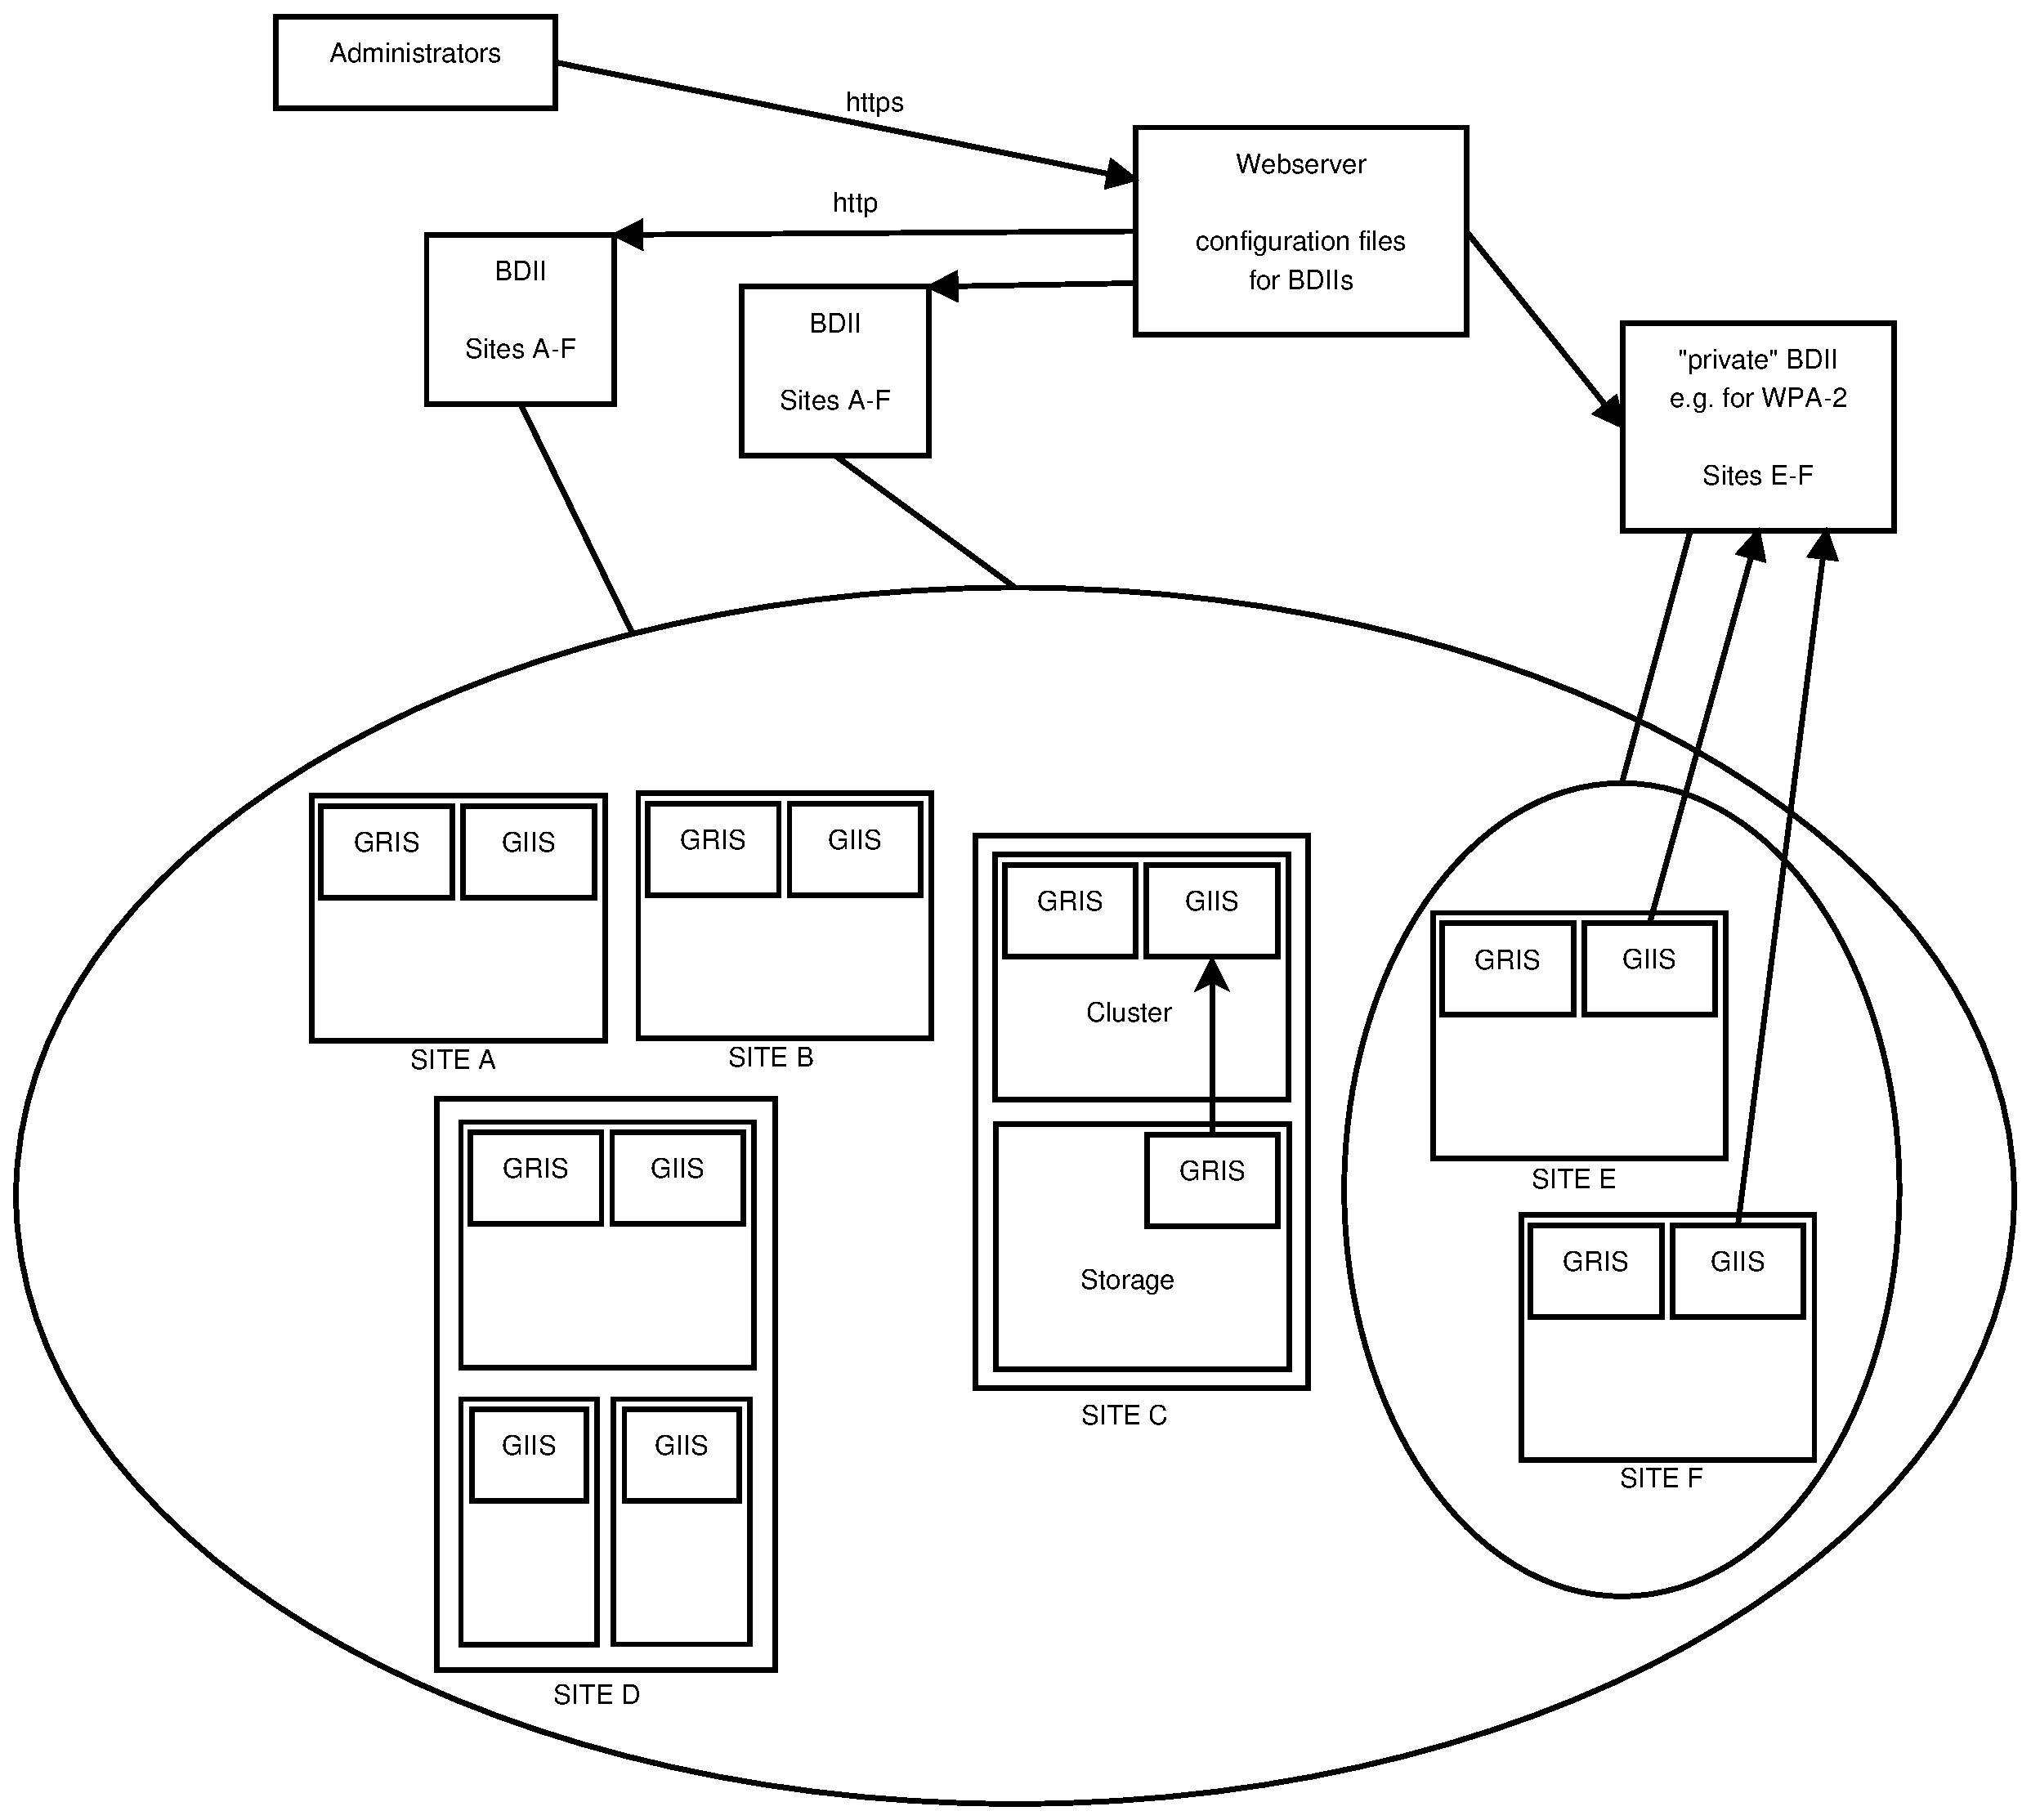
\includegraphics[width=6in]{images/bdii.eps}
\caption{Berkeley Database Information Index}
\label{figure:bdii}
\end{figure}

\section{Performance Monitoring}
%TODO those two paragraphs should be replaced or removed
Standards are being published about the operational models that the grid computing initiative will use. Last decade the EGEE I, II \& III was adopted by european universities to fund and establish a collaborative community of researchers under a central point, the CERN oriented research project in Particle Physics. After EGEE, the European Grid Initiative were formed to lead to the explode of that community into regional initiatives. Performance and availability monitoring tools and views also follow that format, phasing out commonly used SAM \cite{egee3dsa122} and having the adoption of Nagios as the monitoring of regional performance tool.


A taxonomy effort has been made \cite{gerndt2004performance} to present the differences of performance monitoring systems of the grid, and later a more general \cite{zanikolas2007importance} taxonomy paper was published to give a more general visibility of these tools. GridICE was generally used to aggregate the performance metrics of ROCs in high level reports \cite{andreozzi2005gridice}. Later GridICE was left as long as the SAM left, to meet the milestone of EGI to have a regional monitoring tool (Nagios) to report the reliability of the joined sites and report the values for SLA reasons.

\subsection{Ganglia}

Ganglia is a monitoring tool which provides a complete real time monitoring environment. It is used by both academia and industry to monitor large installations of clusters, grids. Any number of host metrics may be monitored in real time using the monitoring core, a multithreaded daemon called Gmond. It runs on every host that is in scope of monitoring. Its four main responsibilities are:

\begin{enumerate}
\item Monitor the changes that happen in the host state
\item Multicast over the network, the changes that has been made
\item Listen to network for changes that other ganglia nodes are multicasting and
\item Answer the status of the whole cluster to specific requests, using XML.
\end{enumerate}

All the data that are gathered of the multicast channel are written to a hash table in memory. The metric data of each node that runs gmond and sends information over the multicast channel are been processed and saved. Data sent over the multicast channel is happening using external data representation (XDR). When there is a request over a TCP connection, the response is in XML.


\begin{figure}[h]
\centering
 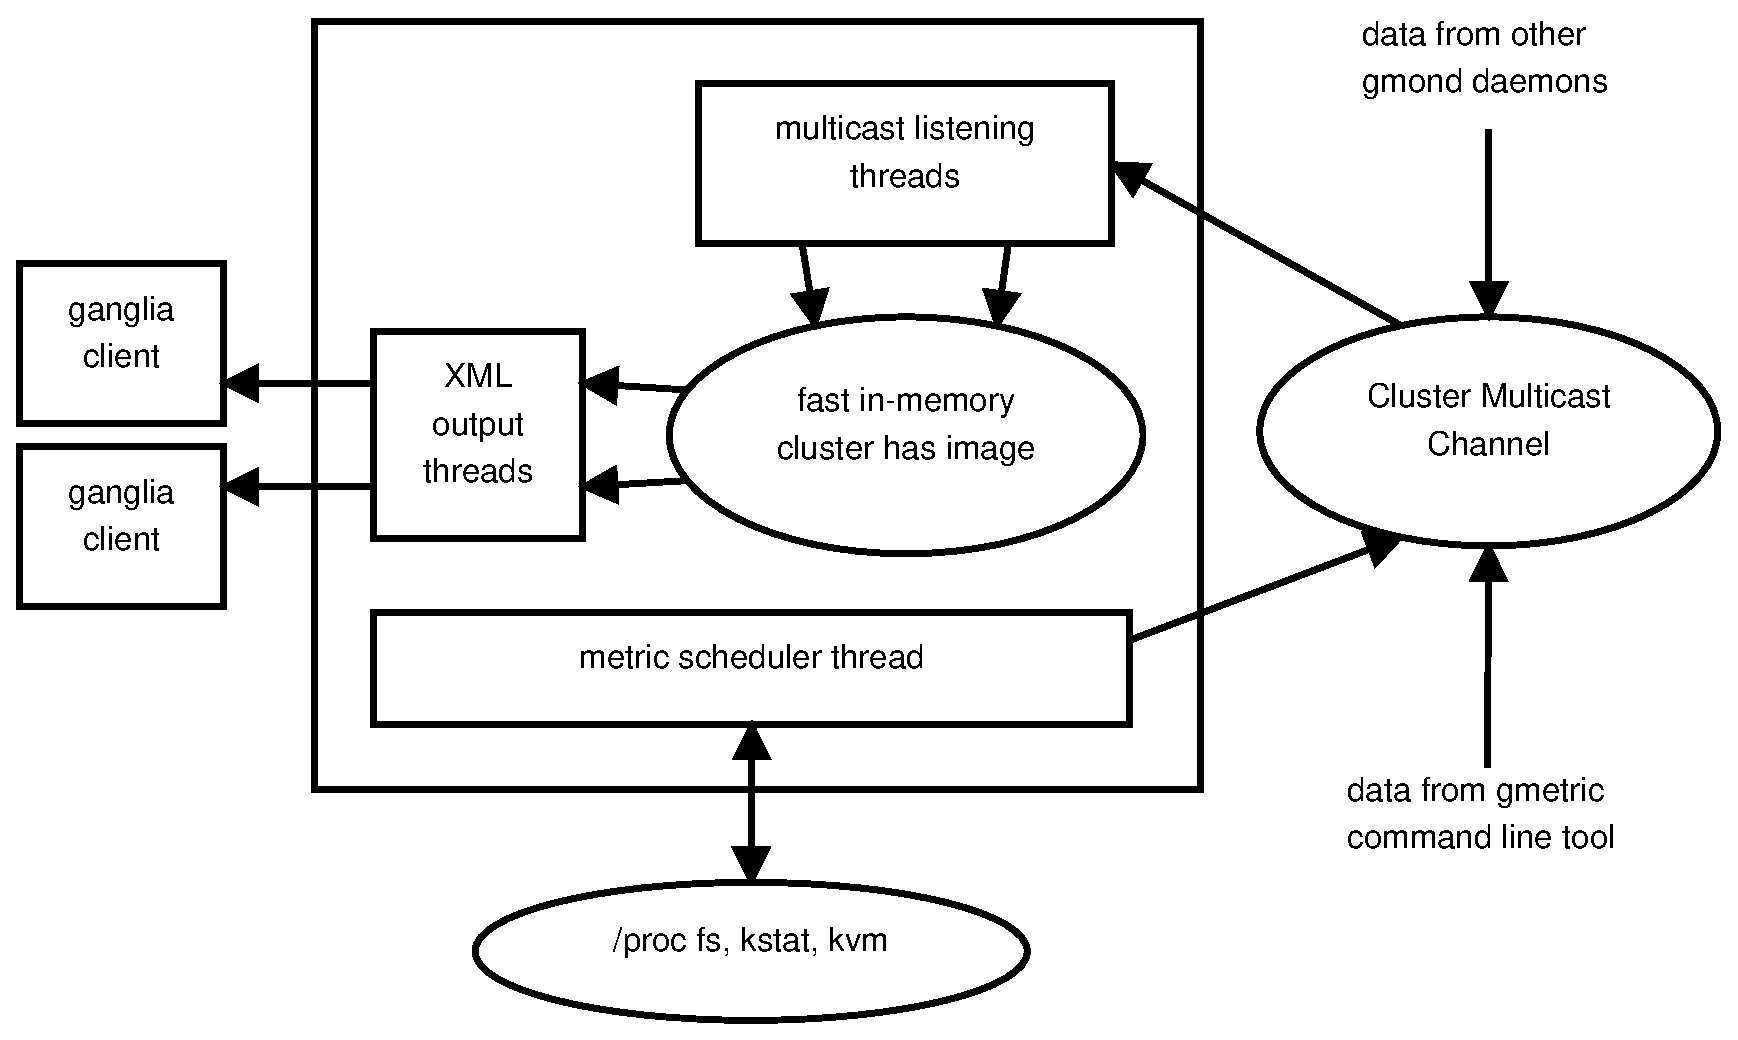
\includegraphics[width=6in]{images/ganglia.eps}
\caption{Ganglia Data Flow}
\label{figure:ganglia}
\end{figure}

\section{European Grid Infrastructure}
Latest EGI directive to form regional operation tools pushed the use of Nagios \cite{imamagic2007grid} as the main tools of availability \& performance (an so reliability) monitoring of the grid. Each NGI/ROC (regional level) has its own interface, and hierarchically there is a Super Nagios interface to report the top level view of general system availability. Nagios offers extensions such as NRPE to remotely invoke check commands in inaccessible/private installations. Another important add-on to Nagios is the NdoUtils, which offers an SQL store of history data to the monitoring interface. Nagios Configuration Generator was introduced to help the automatically generation of the configuration based on the information system of nodes and services. Finally, there has been proposed an integration of SAM views to a Nagios customized interface, to offer the last good known SAM interface to the old users. Nagios also integrates with GGUS, a ticketing system that european grid initiative uses.

% copy-paste apo to egee3dsa122
By the end of the project the monitoring infrastructure (regional Nagios servers and the corresponding regional MyEGEE portals [R52], [R53]) will complete the transition process to a fully distributed infrastructure. The Nagios-based system will totally replace the Service Availability Monitoring (SAM) infrastructure. At the time of writing two monitoring environments are operated: a production one and a test one.


\subsection{NGS}
Brunel University takes part in regional and european initiatives. 5 different Computer Elements exist, and 3 Storage Elements, consisting the UKI-LT2-Brunel site. LT2 stands for London Grid, a co-operation with other London Universities. GridPP and NGS are two collaboration groups that Brunel University is member of, and papers on the web interface \cite{Hobson2007} and real time visualization of the grid status were presented \cite{Huang2007} by GridPP
